% Journal-style test-case article following the VOILAb/JFM writing guide.
\documentclass{jfm}

\usepackage{graphicx}
\usepackage{siunitx}
\usepackage{hyperref}
\usepackage{bm}
\usepackage{booktabs}
\usepackage[noabbrev]{cleveref}

\graphicspath{{figures/}}
\sisetup{detect-all, range-phrase=--, range-units=single}
\hypersetup{
  hidelinks,
  pdftitle={Linear Wave Resistance of an Image-Inspired Displacement Yacht},
  pdfauthor={Ignazio Maria Viola},
  pdfkeywords={sailing yacht, wave resistance, potential flow, Kochin function}
}

\title{Linear Wave Resistance of an Image-Inspired Displacement Yacht}

\author{Ignazio Maria Viola\aff{1,2}
  \corresp{\email{i.m.viola@ed.ac.uk}}}

\affiliation{
\aff{1}School of Engineering, Institute for Energy Systems, University of Edinburgh,
Edinburgh, EH9 3FB, UK,
\aff{2}Department of Industrial Engineering, Alma Mater Studiorum -- University of Bologna,
Bologna, Italy
}

\begin{document}
\maketitle

\begin{abstract}
The wave resistance of displacement sailing yachts changes rapidly when the
Froude number brings the bow- and stern-generated waves into and out of phase.
This paper assesses whether a transparent linear potential-flow method can
resolve this variation for a broad yacht form at early-design cost. The test
case is a generic, fixed-attitude,
\SI{10}{m} hull reconstructed from an undimensioned lines-plan image, with a
beam-to-length ratio of 0.28 and a draft-to-length ratio of 0.06. A
three-dimensional Havelock source distribution is integrated through a Kochin
far-field formulation over Froude numbers from 0.15 to 0.45. The
wave-resistance coefficient increases from 0.00195 at the lowest speed to a
maximum of 0.03859 at a Froude number of 0.425, which corresponds to
\SI{7.61}{kN} for the selected scale. The maximum difference between the fine
and medium hull grids is 1.71\% for Froude numbers greater than or equal to
0.20, while the far-field quadrature tail remains below $5.10\times10^{-4}$.
An independent thin-Wigley benchmark differs from Michell's analytic result by
at most 5.61\%. Far-field maps reveal the associated transition from short,
densely spaced wave crests to longer, more transverse-dominated patterns. The
method therefore resolves useful speed-dependent trends, but its broad-hull
predictions require validation before quantitative design use.
\end{abstract}

\begin{keywords}
sailing yacht, ship waves, wave resistance, potential flow, Kochin function,
hull-form screening
\end{keywords}

\section*{Nomenclature}
\begin{center}
\begin{tabular}{@{}ll@{}}
$a$ & complex Kochin amplitude \\
$C_\mathrm{W}$ & wave-resistance coefficient \\
$Fn$ & Froude number \\
$g$ & gravitational acceleration \\
$I$ & Kochin resistance integral \\
$L$ & reference waterline length \\
$n_x$ & streamwise component of the hull-panel normal \\
$R_\mathrm{W}$ & wave resistance \\
$S$ & wetted surface area \\
$t$ & transverse spectral coordinate \\
$u_\infty$ & magnitude of the free-stream velocity \\
$x,y,z$ & streamwise, transverse and vertical coordinates \\
$\lambda$ & spectral parameter, $\lambda\equiv\sqrt{1+t^2}$ \\
$\rho$ & water density \\
$\sigma$ & source strength \\
$\zeta$ & free-surface elevation or wave-pattern field \\
\end{tabular}
\end{center}

\section{Introduction}\label{sec:introduction}

Wave making is a principal component of the calm-water resistance of a
displacement sailing yacht at moderate and high Froude numbers. It also varies
non-monotonically with speed because waves generated by different parts of the
hull interfere. Michell's thin-ship theory provides the classical linear
description of this process~\citep{Michell1898,Tuck1989}. Havelock subsequently
expressed wave resistance in terms of distributions of singularities beneath
the free surface~\citep{Havelock1932}. These theories remain attractive in
early-stage design because a complete speed sweep can be obtained without the
cost of a viscous free-surface calculation.

The thin-ship assumption is restrictive for sailing yachts, whose immersed
forms may combine a relatively large beam-to-length ratio, rounded sections and
pronounced longitudinal rocker. Rankine-source panel methods retain
three-dimensional geometry and have therefore become a standard route from
classical theory to practical ship-wave computation~\citep{Dawson1977}.
Discretisation can nevertheless distort the propagation of steady ship waves,
and resistance predictions require explicit verification rather than reliance
on a converged linear solve alone~\citep{NakosSclavounos1990}. Three-dimensional
wake spectra have been shown to provide a direct connection between the wave
field and the integrated resistance~\citep{NakosSclavounos1994}.

The present paper addresses the following question: can a compact, transparent
linear source method resolve the speed-dependent resistance and wake topology
of a broad displacement-yacht test case with quantified numerical
sensitivity? To answer it, a generic hull reconstructed from the supplied
lines-plan image is examined over $0.15\leq Fn\leq0.45$. The geometry,
formulation and verification procedure are described in \S\ref{sec:method}.
The resistance curve, numerical diagnostics, far-field spectra and wave
patterns are presented in \S\ref{sec:results}. The implications and limitations
are discussed in \S\ref{sec:discussion}, followed by the conclusions in
\S\ref{sec:conclusions}.

\section{Methodology}\label{sec:method}

The numerical test is designed to isolate wave making. The yacht advances at
constant speed in calm, inviscid, incompressible water of infinite depth. Its
attitude is fixed; sinkage and trim are zero. Appendages and the above-water
geometry are omitted. Dimensional variables are denoted by a hat in this
section. All reported coordinates are nondimensionalised by the waterline
length $\hat L$, velocities by the free-stream speed $\hat u_\infty$ and areas
by $\hat L^2$.

\subsection{Hull geometry and test matrix}\label{subsec:geometry}

The body-fixed frame O$(x,y,z)$ has $x$ increasing from bow to stern, $y$
positive to starboard and $z$ positive upwards. The undisturbed free surface is
$z=0$. The hull is a parametric reconstruction of the principal immersed forms
visible in the supplied raster lines plan. The breadth and draft vary smoothly
between pointed ends, while superelliptic sections reproduce rounded U-shaped
midship sections and increasingly V-shaped forward sections
(\cref{fig:geometry}). Because the source image has no common dimensional
scale, the ratios $B/L=0.28$ and $T/L=0.06$ are imposed independently. The
geometry is therefore a generic displacement yacht rather than a reproduction
of a Dufour 39.

The dimensional reference length is $\hat L=\SI{10}{m}$. The maximum beam and
canoe-body draft are \SI{2.799}{m} and \SI{0.600}{m}, respectively. Numerical
integration of the offsets gives a displaced volume of \SI{7.111}{m^3}, a
seawater displacement of \SI{7289}{kg}, a wetted area of \SI{21.760}{m^2} and a
waterplane area of \SI{17.948}{m^2}. The longitudinal centre of buoyancy is
\SI{0.395}{m} aft of midships. Seawater density is
$\hat\rho=\SI{1025}{kg.m^{-3}}$ and gravitational acceleration is
$\hat g=\SI{9.80665}{m.s^{-2}}$.

\begin{figure}
\begin{center}
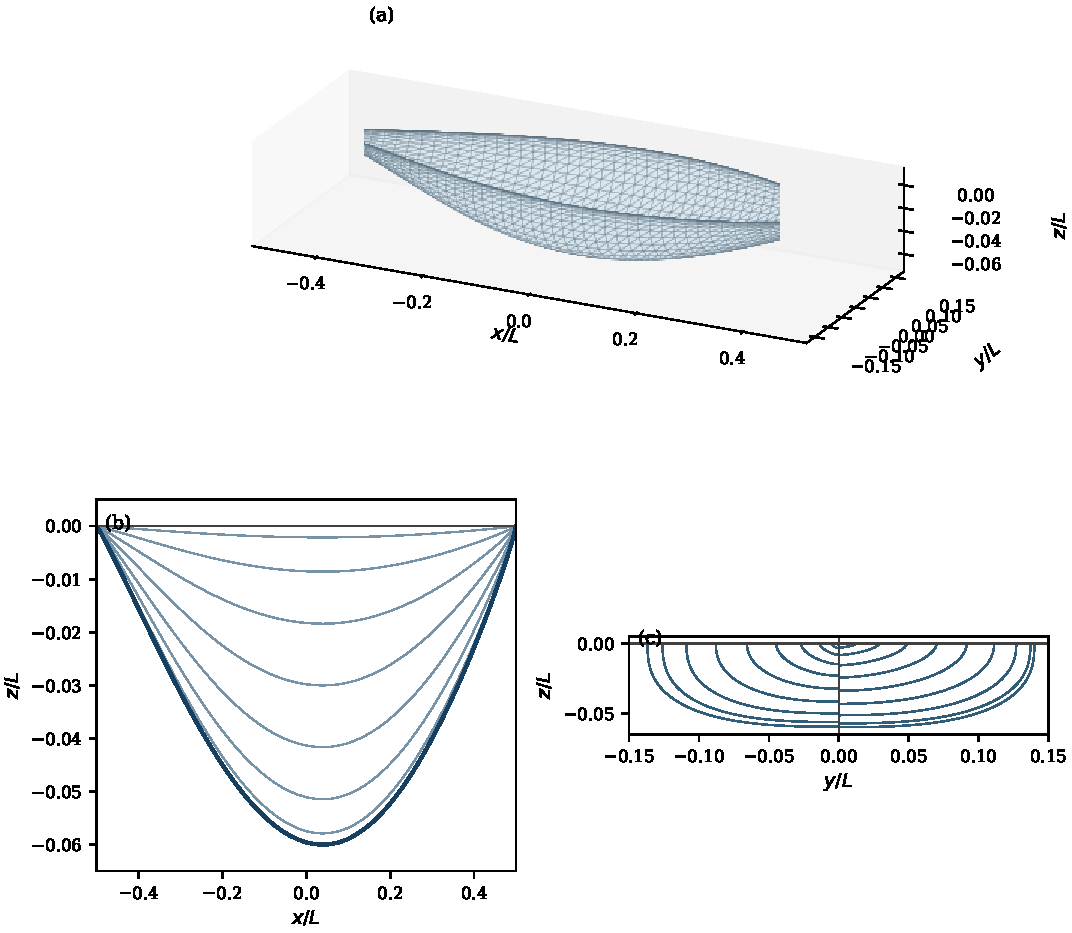
\includegraphics[width=0.96\textwidth]{hull_geometry.pdf}
\caption{Image-inspired displacement-yacht geometry: (a) fine triangular
surface mesh, (b) profile and longitudinal section lines, and (c) body plan with aft sections
on the left and forward sections on the right. The waterline is $z/L=0$.}
\label{fig:geometry}
\end{center}
\end{figure}

The Froude number is
\begin{equation}\label{eq:froude}
Fn\equiv\frac{\hat u_\infty}{\sqrt{\hat g\hat L}}.
\end{equation}
Thirteen operating points are evaluated at increments of 0.025 over
$0.15\leq Fn\leq0.45$, corresponding to speeds from \SI{1.486}{m.s^{-1}} to
\SI{4.456}{m.s^{-1}}. Six operating points, $Fn=0.20$, 0.25, 0.30, 0.35,
0.40 and 0.45, are selected for wave-pattern analysis.

\subsection{Linear potential-flow formulation}\label{subsec:formulation}

The disturbance potential $\phi$ satisfies Laplace's equation. On the mean
hull surface and mean free surface, respectively, the linear boundary
conditions are
\begin{equation}\label{eq:boundary_conditions}
\bm{\nabla}\phi\bm{\cdot}\bm{n}=-n_x,
\qquad Fn^2\frac{\partial^2\phi}{\partial x^2}
+\frac{\partial\phi}{\partial z}=0\quad(z=0),
\end{equation}
with an upstream radiation condition. The robust resistance path uses the
linearised Havelock source distribution $\sigma_j=-n_{x,j}$ on each actual
three-dimensional hull panel. Hence, finite breadth, depth, area and transverse
phase are retained, although the source strength is linearised.

For the transverse spectral coordinate $t$, the wavenumber components are
\begin{equation}\label{eq:wavenumbers}
\lambda\equiv\sqrt{1+t^2},\qquad
k_x\equiv\frac{\lambda}{Fn^2},\qquad
k_y\equiv\frac{\lambda t}{Fn^2},\qquad
k\equiv\frac{\lambda^2}{Fn^2}.
\end{equation}
Analytical reflection of the starboard half hull gives the Kochin amplitude
\begin{equation}\label{eq:kochin_amplitude}
a(t)\equiv-\sum_j\sigma_j\Delta S_j
\exp\left(kz_j-\mathrm{i}k_xx_j\right)\cos(k_yy_j),
\end{equation}
where $\mathrm{i}\equiv\sqrt{-1}$. The positive-definite resistance integral
and the wetted-area-normalised wave-resistance coefficient are
\begin{equation}\label{eq:resistance_integral}
I\equiv\int_0^\infty\lambda|a(t)|^2\,\mathrm{d}t,
\qquad
C_\mathrm{W}\equiv\frac{8I}{\pi Fn^4(S/L^2)}.
\end{equation}
This normalisation is equivalent to
\begin{equation}\label{eq:dimensional_resistance}
\hat R_\mathrm{W}\equiv
\frac{1}{2}\hat\rho\hat u_\infty^2\hat S C_\mathrm{W}.
\end{equation}

The integral is evaluated on 6001 quadrature points after the transformation
$t=q^2$, with $0\leq t\leq60$. The contribution from the final 20\% of the
interval divided by $I$ is reported as the quadrature-tail indicator. The full
implementation and machine-readable outputs are distributed with the
article~\citep{Viola2026}.

\subsection{Far-field wave-pattern reconstruction}\label{subsec:wave_pattern}

The Kochin spectrum is also used to visualise the radiating far field. This
avoids presenting the compact free-surface-panel solution as a converged local
elevation. The plotted field is
\begin{equation}\label{eq:pattern}
\zeta_\mathrm{N}(x,y)\equiv
\frac{\Real\left\{\int_0^{12}w(t)\lambda a(t)
\exp(\mathrm{i}k_xx)\cos(k_yy)\,\mathrm{d}t\right\}}
{\displaystyle\max_{x,y}\left|\Real\left\{\int_0^{12}w(t)\lambda a(t)
\exp(\mathrm{i}k_xx)\cos(k_yy)\,\mathrm{d}t\right\}\right|},
\end{equation}
where $w=1$ for $t\leq9.6$ and decreases to zero through a raised-cosine taper
at $t=12$. Each operating point is normalised independently. Consequently,
\cref{eq:pattern} shows phase, wavelength and interference topology, but not
the variation of dimensional wave amplitude between speeds. Wave-pattern
resistance inferred from measured longitudinal cuts is a useful independent
validation quantity~\citep{ITTC2021}; no such measurements are available for
the present synthetic hull.

\subsection{Solution verification and numerical sensitivity}\label{subsec:verification}

Implementation verification uses a Wigley hull with $B/L=0.05$ and
$T/L=0.0625$. Its slenderness permits an independent analytic evaluation of
Michell's integral. The 41 by 15 point panel solution differs from the analytic
coefficient by 2.50--5.61\% over $0.20\leq Fn\leq0.40$
(\cref{fig:wigley_verification}). This comparison verifies the normalisation,
surface integration and spectral quadrature in the limit for which the
reference theory applies; it does not validate the broad yacht case.

\begin{figure}
\begin{center}
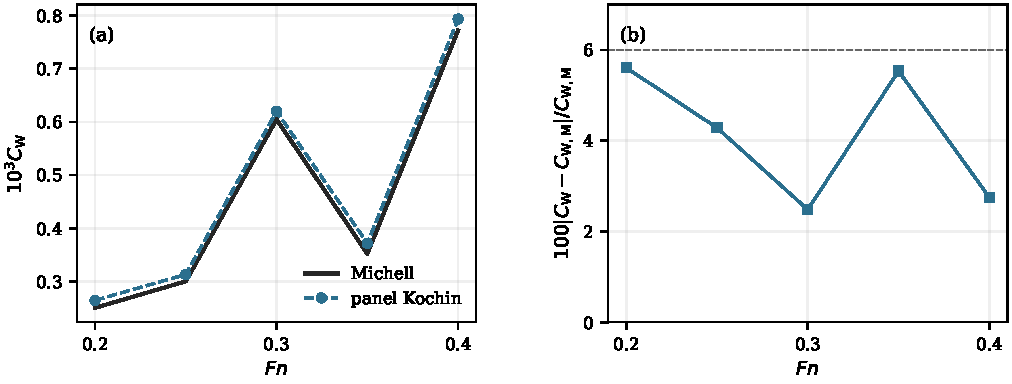
\includegraphics[width=0.94\textwidth]{wigley_verification.pdf}
\caption{Wigley thin-limit verification: (a) wave-resistance coefficient from
the panel Kochin integral and independent Michell evaluation; (b) absolute
relative difference, with the dashed line marking 6\%. Here $B/L=0.05$ and
$T/L=0.0625$.}
\label{fig:wigley_verification}
\end{center}
\end{figure}

The yacht is discretised with coarse, medium and fine half-hull grids of 31 by
13, 41 by 15 and 51 by 19 points. Degenerate triangles at the stem, stern and
centreline are removed, leaving 696, 1092 and 1764 active panels. The absolute
fine-to-medium difference divided by the fine result is used as a
discretisation-sensitivity estimate. A formal grid convergence index is not
reported because the two surface directions do not have one common refinement
factor and the lowest-speed response is not monotonically converged. This
choice separates a directly observed sensitivity from a statistical or
asymptotic uncertainty estimate~\citep{EcaHoekstra2014}.

\section{Results}\label{sec:results}

\subsection{Wave resistance}\label{subsec:resistance_results}

The three grids give visually coincident resistance curves over most of the
speed range (\cref{fig:resistance}a). The coefficient increases from 0.001951
at $Fn=0.15$ to 0.007616 at $Fn=0.275$, decreases slightly to 0.007586 at
$Fn=0.30$, and then rises steeply. It reaches a maximum of 0.038591 at
$Fn=0.425$ before decreasing to 0.037686 at $Fn=0.45$. The hollow near
$Fn=0.30$ and the high-speed crest are consistent with destructive and
constructive interference between longitudinally separated source regions.

\begin{figure}
\begin{center}
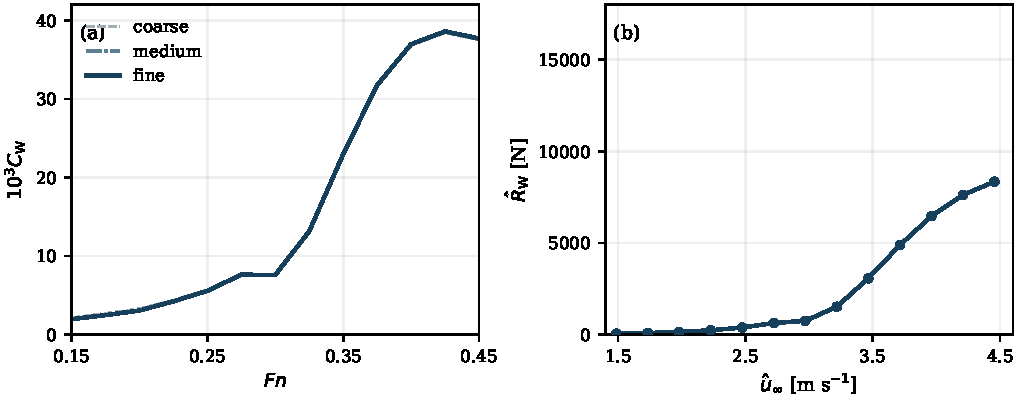
\includegraphics[width=0.98\textwidth]{resistance_convergence.pdf}
\caption{Wave resistance versus speed: (a) area-normalised coefficient for the
three hull grids; (b) dimensional resistance for the fine grid and the
\SI{10}{m} test case in seawater.}
\label{fig:resistance}
\end{center}
\end{figure}

At the selected scale, the maximum coefficient occurs at
$\hat u_\infty=\SI{4.209}{m.s^{-1}}$ and gives
$\hat R_\mathrm{W}=\SI{7.613}{kN}$ (\cref{fig:resistance}b). The dimensional
resistance continues to increase at $Fn=0.45$, despite the slight decrease in
coefficient, because the dynamic pressure is proportional to speed squared.
This result is wave resistance alone and must not be interpreted as the total
calm-water resistance.

\subsection{Numerical diagnostics}\label{subsec:numerical_results}

The fine-to-medium difference is below 1.71\% for every case with
$Fn\geq0.20$, and its mean is 0.36\% over this subset
(\cref{fig:numerical_diagnostics}a). The difference rises to 3.45\% at
$Fn=0.15$, where the shorter waves demand greater longitudinal resolution.
The reported curve should therefore be considered less resolved at the lower
boundary of the declared envelope.

\begin{figure}
\begin{center}
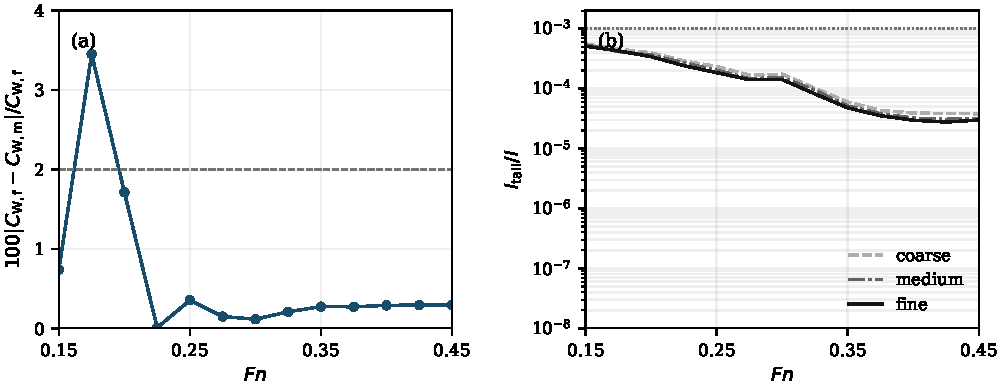
\includegraphics[width=0.96\textwidth]{numerical_diagnostics.pdf}
\caption{Numerical diagnostics versus Froude number: (a) absolute fine-to-medium
relative difference in wave-resistance coefficient; (b) final-20\% Kochin
quadrature contribution for each grid, with the dotted line marking
$I_\mathrm{tail}/I=10^{-3}$.}
\label{fig:numerical_diagnostics}
\end{center}
\end{figure}

The quadrature tail remains below $5.10\times10^{-4}$ for the fine grid and
below $5.55\times10^{-4}$ across all three grids
(\cref{fig:numerical_diagnostics}b). The largest values occur at the two lowest
Froude numbers. These indicators show that the finite Kochin interval contains
the computed spectrum to the prescribed tolerance, independently of the hull
grid comparison.

\subsection{Kochin spectra and wave patterns}\label{subsec:pattern_results}

The normalised integrand $\lambda|a|^2$ changes systematically with speed
(\cref{fig:spectra}). At the lower Froude numbers, several comparable peaks
extend over the resolved transverse spectrum. Increasing the Froude number
concentrates the dominant contribution towards smaller $t$, while secondary
lobes retain the signature of bow--stern interference. The concentration is
particularly strong at $Fn=0.40$ and 0.45, where the dominant low-$t$ content
coincides with the crest of the resistance curve.

\begin{figure}
\begin{center}
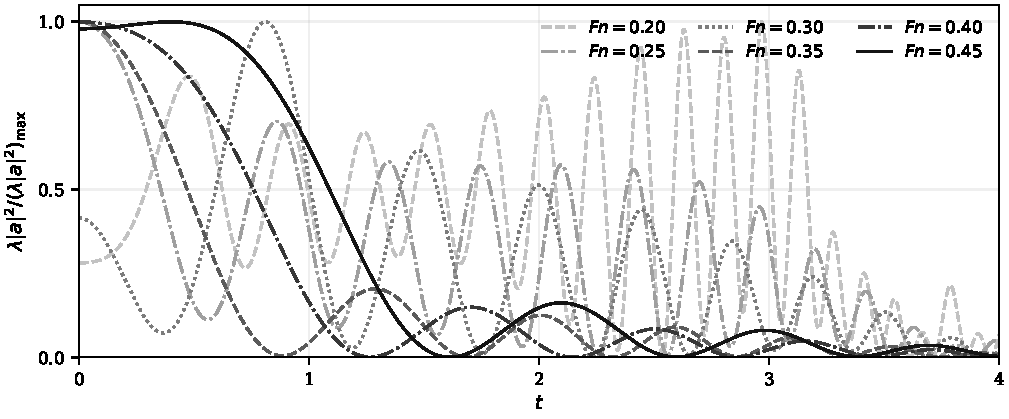
\includegraphics[width=0.96\textwidth]{kochin_spectra.pdf}
\caption{Normalised Kochin resistance-integrand density versus transverse
spectral coordinate for six Froude numbers. Each curve is divided by its own
maximum to expose changes in spectral distribution.}
\label{fig:spectra}
\end{center}
\end{figure}

The far-field maps translate these spectra into physical-space topology
(\cref{fig:wave_patterns}). At $Fn=0.20$, the wake contains closely spaced,
high-angle divergent crests. The characteristic spacing increases from
$Fn=0.25$ to 0.30, while alternating bands reveal interference between the
forward and aft source regions. At $Fn=0.35$, a stronger long-wave component
appears immediately downstream and extends into coherent oblique arms. The
$Fn=0.40$ and 0.45 patterns are dominated by longer waves and broader
transverse bands, consistent with their low-$t$ spectra.

\begin{figure}
\begin{center}
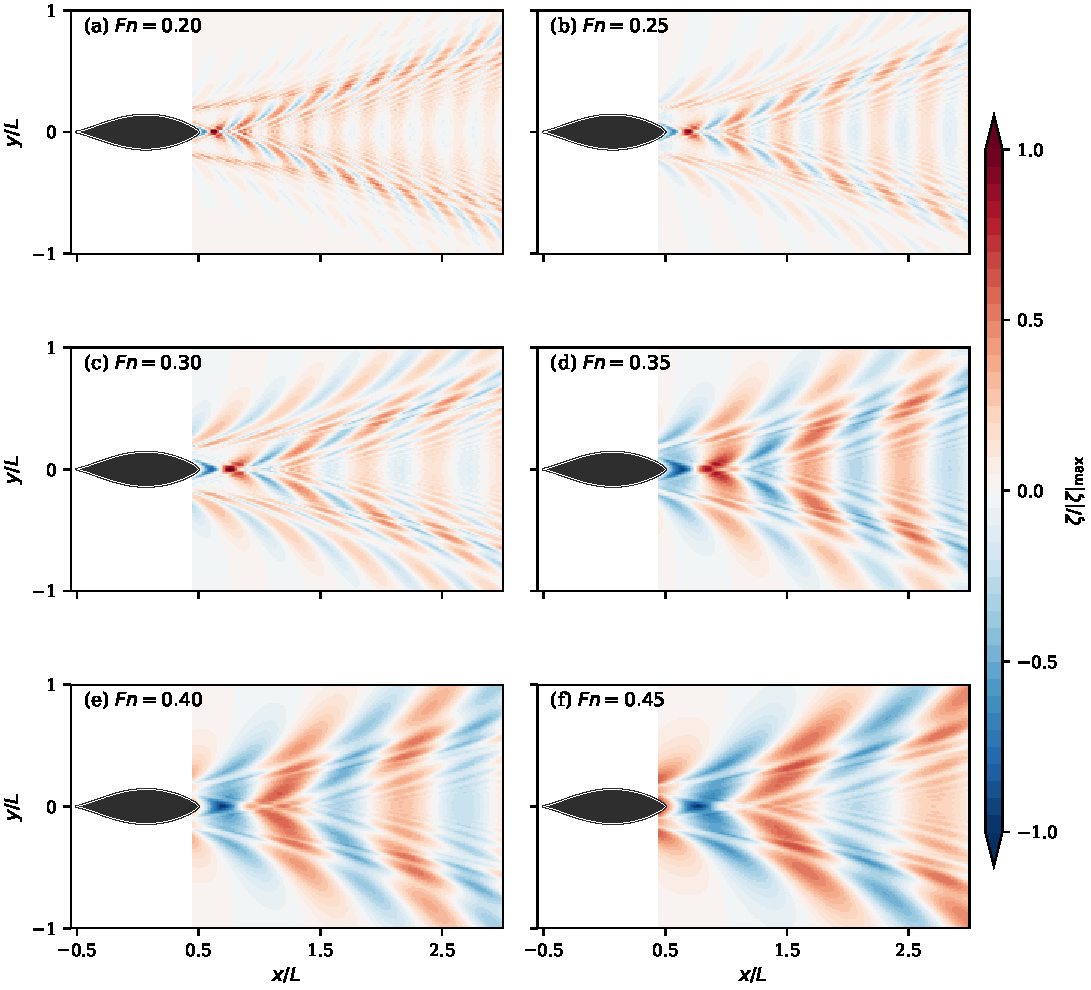
\includegraphics[width=0.97\textwidth]{wave_patterns.pdf}
\caption{Normalised far-field wave-pattern phase for (a) $Fn=0.20$, (b) 0.25,
(c) 0.30, (d) 0.35, (e) 0.40 and (f) 0.45. Red and blue denote opposite phases;
each field is independently normalised and therefore does not compare wave
amplitudes between Froude numbers. Flow and vessel motion are towards positive
$x$.}
\label{fig:wave_patterns}
\end{center}
\end{figure}

The maps are symmetric about the centreplane because only upright, zero-leeway
motion is considered. They remain confined to the classical radiating wake and
show no breaking, viscous attenuation or near-field crest steepening. The
visual progression nevertheless explains why a scalar resistance curve alone
is insufficient: similar coefficients can result from materially different
distributions of wave direction and phase.

\section{Discussion}\label{sec:discussion}

The test supports the thesis that a low-order three-dimensional source method
can resolve useful speed-dependent trends for a displacement-yacht form. The
positive Kochin integral prevents a non-physical negative resistance, the
three-grid comparison bounds the observed discretisation sensitivity, and the
far-field reconstruction provides a direct qualitative explanation of the
humps and hollow. A complete thirteen-point fine-grid sweep, including figures
and machine-readable output, is reproducible with one Python script.

The numerical evidence has clear boundaries. First, the imposed source
strength is a linear Neumann--Kelvin approximation. The test hull has
$B/L=0.28$ and is therefore substantially broader than the Wigley verification
body. The 5.61\% benchmark error must not be transferred as an uncertainty for
the yacht. Secondly, the fixed-attitude model omits dynamic sinkage and trim,
which can shift interference features. Thirdly, viscosity, boundary-layer
growth, separation, appendage drag, wave breaking and transom ventilation are
absent. Finally, the plotted wave fields are independently normalised
far-field phase reconstructions rather than dimensional near-field elevations.

The resistance level, especially the high-speed coefficient, should therefore
be interpreted as a screening prediction. Quantitative design use requires a
like-for-like towing-tank or validated viscous free-surface computation. The
most informative experiment would measure both resistance and longitudinal
wave cuts at the same fixed attitude. That combination permits direct
comparison of the scalar force, the wave spectrum and the spatial pattern in
accordance with the International Towing Tank Conference procedure
~\citep{ITTC2021}.

\section{Conclusions}\label{sec:conclusions}

A linear potential-flow test has been performed for a broad, image-inspired
displacement yacht over Froude numbers from 0.15 to 0.45. The method represents
the three-dimensional immersed surface with sources and obtains wave
resistance from a positive far-field energy integral. A ten-metre hull in
seawater provides the dimensional reference.

The calculation resolves a shallow resistance hollow near a Froude number of
0.30 followed by a pronounced high-speed rise. The wave-resistance coefficient
reaches 0.03859 at a Froude number of 0.425, corresponding to 7.61 kilonewtons
at the selected scale. Medium-to-fine grid differences remain below 1.71 per
cent from a Froude number of 0.20 upwards, and the unresolved tail of the
far-field integral remains below 0.051 per cent. The associated wave patterns
change from densely spaced divergent crests to longer patterns dominated by
broad transverse bands.

These results demonstrate that the method is suitable for rapid, internally
consistent comparisons of displacement-yacht hull forms and operating speeds.
They do not establish predictive accuracy for a real yacht. The principal
limitations are the linearised source strength, fixed attitude, inviscid flow
and absence of experimental validation. The next step is a controlled
comparison with resistance and wave-cut measurements for a fully specified
hull geometry.

\section*{Acknowledgements}

The computational test uses the hull-form image supplied for this project. No
external experimental data were used.

\section*{Declaration of interests}

The Author reports no conflict of interest.

\section*{Data availability statement}

The source code, exact test-case script, tabulated resistance curve, wave fields
and all figure sources are available in the
\href{https://github.com/ignaziomviola/wave-resistance/tree/codex/displacement-yacht-bem}{project repository}.
The calculation is reproduced from the repository root with
\texttt{python examples/journal\_test\_case.py}; the manuscript is compiled
with \texttt{latexmk -pdf article/main.tex}.

\bibliographystyle{jfm}
\bibliography{references}

\end{document}
